% $Header: /cvsroot/latex-beamer/latex-beamer/solutions/generic-talks/generic-ornate-15min-45min.en.tex,v 1.5 2007/01/28 20:48:23 tantau Exp $

\documentclass{beamer}
\usepackage{pdfpages}
\usepackage{booktabs}
%%%%%%%%%%%%%%%%%%%%%%%%%%%%%%%%%%%%%%%%%%%%%%%%%%%%%%%%%%%%%%%%%%%%%%%%%
%%%%%%%%%%%%  UJV template %%%%%%%%%%%%%%%%%%%%%%%%%%%%%%%%%%%%%%%%%%%%%%
%%%%%%%%%%%%%%%%%%%%%%%%%%%%%%%%%%%%%%%%%%%%%%%%%%%%%%%%%%%%%%%%%%%%%%%%%
%%%%%%% %%%%%%%%%%%%%%%%%%%%%%%%%%%%%%%%%%%%%%%%%%%%%%%%%%%%%%%%%%%%%%%%%%%%%%%%%
%%%%%%%%%%%%  UJV template %%%%%%%%%%%%%%%%%%%%%%%%%%%%%%%%%%%%%%%%%%%%%%
%%%%%%%%%%%%%%%%%%%%%%%%%%%%%%%%%%%%%%%%%%%%%%%%%%%%%%%%%%%%%%%%%%%%%%%%%
%%%%%%% %%%%%%%%%%%%%%%%%%%%%%%%%%%%%%%%%%%%%%%%%%%%%%%%%%%%%%%%%%%%%%%%%%%%%%%%%
%%%%%%%%%%%%  UJV template %%%%%%%%%%%%%%%%%%%%%%%%%%%%%%%%%%%%%%%%%%%%%%
%%%%%%%%%%%%%%%%%%%%%%%%%%%%%%%%%%%%%%%%%%%%%%%%%%%%%%%%%%%%%%%%%%%%%%%%%
%%%%%%% \input{ujvtemplate.tex} somewhere after documentclass %%%%%%%%%%
%%%%%%%%%%%%%%%%%%%%%%%%%%%%%%%%%%%%%%%%%%%%%%%%%%%%%%%%%%%%%%%%%%%%%%%%%

\usepackage{graphicx}
\usepackage{ifthen}
\usepackage{tikz}
\usefonttheme{professionalfonts}
\usepackage{times}
\usepackage{amsmath}
\usetikzlibrary{arrows,shapes}
\usetikzlibrary{decorations.pathmorphing}

\definecolor{ujvdarkblue}{rgb}{0,0.33,0.647} 
\definecolor{ujvlightblue}{rgb}{0,0.607,0.788} 

\mode<presentation>

{

\usetheme{default}
%\usetheme{boxes}
}


\setbeamertemplate{frametitle}{
\vspace*{2.5mm}\hspace*{-1mm}\insertframetitle}

\setbeamertemplate{headline}
{
  \leavevmode%
  \hbox{%
  \begin{beamercolorbox}[wd=.5\paperwidth,ht=2.25ex,dp=1ex,right,rightskip=1em]{section in head/foot}%
    \usebeamerfont{subsection in head/foot}\hspace*{2ex}\color{ujvlightblue}{\insertshorttitle}
  \end{beamercolorbox}%
  \begin{beamercolorbox}[wd=.5\paperwidth,ht=2.25ex,dp=1ex,left,leftskip=1em]{subsection in head/foot}%
    \usebeamerfont{section in head/foot}\color{ujvdarkblue}{\insertsectionhead}\hspace*{2ex}
  \end{beamercolorbox}}%
  \vskip0pt%
}


\useinnertheme{rounded}
\usecolortheme{orchid}
\usefonttheme{default}

%\newcommand{\Ffootline}{%
%\insertsection % The left end of the footline
%\hfill
%\textit{Moo} % The center
%\hfill
%\insertframenumber/\inserttotalframenumber} % And the right end

\newcommand{\Ffootline}{%
\color[rgb]{1,1,1}\bf\tiny\insertframenumber % The left end of the footline
\hfill
} % And the right end


\setbeamertemplate{footline}{%
\usebeamerfont{structure}
\begin{beamercolorbox}[wd=\paperwidth,ht=2.25ex,dp=1ex]{title in head/foot}%
\ifnum\insertframenumber<10\relax%
\Tiny\vspace*{3.6mm}\hspace*{9.5mm} \Ffootline \hspace{8mm}
\fi
\ifnum\insertframenumber>9\relax%
\Tiny\vspace*{3.6mm}\hspace*{8.9mm} \Ffootline \hspace{8mm}
\fi
\end{beamercolorbox}}

\setbeamertemplate{itemize/enumerate body begin}{\setlength{\leftmargini}{11pt}}

\setbeamertemplate{sections/subsections in toc}[square]

\defbeamertemplate{itemize item}{image}{\small\raisebox{0.2ex}{
\includegraphics[height=1.ex]{fig_item1}}}
\defbeamertemplate{itemize subitem}{image}{\scriptsize\raisebox{0.2ex}{
\includegraphics[height=1.ex]{fig_item2}}}
\defbeamertemplate{itemize subsubitem}{image}{\tiny\raisebox{0.2ex}{
\includegraphics[height=1.0ex]{fig_item2}}}
%\defbeamertemplate{enumerate item}{image}{\small\raisebox{0.0ex}{
\includegraphics[height=0.5ex]{fig_item1.png}}\hspace*{-1ex}\theenumi}

\setbeamertemplate{itemize item}[image]
\setbeamertemplate{itemize subitem}[image]
\setbeamertemplate{itemize subsubitem}[image]

\setbeamertemplate{enumerate items}[square]
%\newcommand{\ujvitem}[0]{
\includegraphics[height=1.6 ex]{fig_item1.png}}
%\setbeamertemplate{enumerate items}{
%                             \hspace{0.5ex}\ujvitem
%\usebeamercolor[fg]{item projected}  \footnotesize   
%                            \hspace*{-1ex}\raisebox{1.5pt}{\theenumi}     
%                            }


\definecolor{ujvdarkblue}{rgb}{0,0.33,0.647} 
\definecolor{ujvlightblue}{rgb}{0,0.607,0.788} 
\setbeamercolor{frametitle}{fg=ujvdarkblue}
\setbeamercolor{title}{fg=ujvdarkblue}
\setbeamercolor{structure}{fg=ujvdarkblue}
\setbeamercolor{block title}{use=structure,fg=white,bg=ujvdarkblue}

\usebackgroundtemplate{
    
\includegraphics[width=\paperwidth,height=\paperheight]{fig_bacground}
}


\mode<all>


\pgfdeclareimage[width=\paperwidth]{mybackground}{fig_bacground0}

\defbeamertemplate*{title page}{customized}[1][]{
  
  \begin{picture}(0,0)
    
    \put(-40,-165){%
      \pgfuseimage{mybackground}
    }
    
    \put(110,-70){%
      \begin{minipage}{6.7cm}
          \color{ujvdarkblue}{
            \usebeamerfont{title}{\bf\flushright\inserttitle\par}
            \vspace{0.2cm}
            \usebeamerfont{author}\hfill\insertauthor\par
            \vspace{0.2cm}
            \usebeamerfont{institute}\hfill\insertinstitute\par
            \vspace{0.2cm}
            \usebeamerfont{date}\hfill\insertdate\par
          }
      \end{minipage}
 }       
  \end{picture}
  
}



%%%%%%%%%%%%%%%%%%%%%%%%%%%%%%%%%%%%%%%%%%%%%%%%%%%%%%%%%%%%%%%%%%%%%%%%%
%%%%%%%%%%%%  UJV template  END %%%%%%%%%%%%%%%%%%%%%%%%%%%%%%%%%%%%%%%%%
%%%%%%%%%%%%%%%%%%%%%%%%%%%%%%%%%%%%%%%%%%%%%%%%%%%%%%%%%%%%%%%%%%%%%%%%%
 somewhere after documentclass %%%%%%%%%%
%%%%%%%%%%%%%%%%%%%%%%%%%%%%%%%%%%%%%%%%%%%%%%%%%%%%%%%%%%%%%%%%%%%%%%%%%

\usepackage{graphicx}
\usepackage{ifthen}
\usepackage{tikz}
\usefonttheme{professionalfonts}
\usepackage{times}
\usepackage{amsmath}
\usetikzlibrary{arrows,shapes}
\usetikzlibrary{decorations.pathmorphing}

\definecolor{ujvdarkblue}{rgb}{0,0.33,0.647} 
\definecolor{ujvlightblue}{rgb}{0,0.607,0.788} 

\mode<presentation>

{

\usetheme{default}
%\usetheme{boxes}
}


\setbeamertemplate{frametitle}{
\vspace*{2.5mm}\hspace*{-1mm}\insertframetitle}

\setbeamertemplate{headline}
{
  \leavevmode%
  \hbox{%
  \begin{beamercolorbox}[wd=.5\paperwidth,ht=2.25ex,dp=1ex,right,rightskip=1em]{section in head/foot}%
    \usebeamerfont{subsection in head/foot}\hspace*{2ex}\color{ujvlightblue}{\insertshorttitle}
  \end{beamercolorbox}%
  \begin{beamercolorbox}[wd=.5\paperwidth,ht=2.25ex,dp=1ex,left,leftskip=1em]{subsection in head/foot}%
    \usebeamerfont{section in head/foot}\color{ujvdarkblue}{\insertsectionhead}\hspace*{2ex}
  \end{beamercolorbox}}%
  \vskip0pt%
}


\useinnertheme{rounded}
\usecolortheme{orchid}
\usefonttheme{default}

%\newcommand{\Ffootline}{%
%\insertsection % The left end of the footline
%\hfill
%\textit{Moo} % The center
%\hfill
%\insertframenumber/\inserttotalframenumber} % And the right end

\newcommand{\Ffootline}{%
\color[rgb]{1,1,1}\bf\tiny\insertframenumber % The left end of the footline
\hfill
} % And the right end


\setbeamertemplate{footline}{%
\usebeamerfont{structure}
\begin{beamercolorbox}[wd=\paperwidth,ht=2.25ex,dp=1ex]{title in head/foot}%
\ifnum\insertframenumber<10\relax%
\Tiny\vspace*{3.6mm}\hspace*{9.5mm} \Ffootline \hspace{8mm}
\fi
\ifnum\insertframenumber>9\relax%
\Tiny\vspace*{3.6mm}\hspace*{8.9mm} \Ffootline \hspace{8mm}
\fi
\end{beamercolorbox}}

\setbeamertemplate{itemize/enumerate body begin}{\setlength{\leftmargini}{11pt}}

\setbeamertemplate{sections/subsections in toc}[square]

\defbeamertemplate{itemize item}{image}{\small\raisebox{0.2ex}{
\includegraphics[height=1.ex]{fig_item1}}}
\defbeamertemplate{itemize subitem}{image}{\scriptsize\raisebox{0.2ex}{
\includegraphics[height=1.ex]{fig_item2}}}
\defbeamertemplate{itemize subsubitem}{image}{\tiny\raisebox{0.2ex}{
\includegraphics[height=1.0ex]{fig_item2}}}
%\defbeamertemplate{enumerate item}{image}{\small\raisebox{0.0ex}{
\includegraphics[height=0.5ex]{fig_item1.png}}\hspace*{-1ex}\theenumi}

\setbeamertemplate{itemize item}[image]
\setbeamertemplate{itemize subitem}[image]
\setbeamertemplate{itemize subsubitem}[image]

\setbeamertemplate{enumerate items}[square]
%\newcommand{\ujvitem}[0]{
\includegraphics[height=1.6 ex]{fig_item1.png}}
%\setbeamertemplate{enumerate items}{
%                             \hspace{0.5ex}\ujvitem
%\usebeamercolor[fg]{item projected}  \footnotesize   
%                            \hspace*{-1ex}\raisebox{1.5pt}{\theenumi}     
%                            }


\definecolor{ujvdarkblue}{rgb}{0,0.33,0.647} 
\definecolor{ujvlightblue}{rgb}{0,0.607,0.788} 
\setbeamercolor{frametitle}{fg=ujvdarkblue}
\setbeamercolor{title}{fg=ujvdarkblue}
\setbeamercolor{structure}{fg=ujvdarkblue}
\setbeamercolor{block title}{use=structure,fg=white,bg=ujvdarkblue}

\usebackgroundtemplate{
    
\includegraphics[width=\paperwidth,height=\paperheight]{fig_bacground}
}


\mode<all>


\pgfdeclareimage[width=\paperwidth]{mybackground}{fig_bacground0}

\defbeamertemplate*{title page}{customized}[1][]{
  
  \begin{picture}(0,0)
    
    \put(-40,-165){%
      \pgfuseimage{mybackground}
    }
    
    \put(110,-70){%
      \begin{minipage}{6.7cm}
          \color{ujvdarkblue}{
            \usebeamerfont{title}{\bf\flushright\inserttitle\par}
            \vspace{0.2cm}
            \usebeamerfont{author}\hfill\insertauthor\par
            \vspace{0.2cm}
            \usebeamerfont{institute}\hfill\insertinstitute\par
            \vspace{0.2cm}
            \usebeamerfont{date}\hfill\insertdate\par
          }
      \end{minipage}
 }       
  \end{picture}
  
}



%%%%%%%%%%%%%%%%%%%%%%%%%%%%%%%%%%%%%%%%%%%%%%%%%%%%%%%%%%%%%%%%%%%%%%%%%
%%%%%%%%%%%%  UJV template  END %%%%%%%%%%%%%%%%%%%%%%%%%%%%%%%%%%%%%%%%%
%%%%%%%%%%%%%%%%%%%%%%%%%%%%%%%%%%%%%%%%%%%%%%%%%%%%%%%%%%%%%%%%%%%%%%%%%
 somewhere after documentclass %%%%%%%%%%
%%%%%%%%%%%%%%%%%%%%%%%%%%%%%%%%%%%%%%%%%%%%%%%%%%%%%%%%%%%%%%%%%%%%%%%%%

\usepackage{graphicx}
\usepackage{ifthen}
\usepackage{tikz}
\usefonttheme{professionalfonts}
\usepackage{times}
\usepackage{amsmath}
\usetikzlibrary{arrows,shapes}
\usetikzlibrary{decorations.pathmorphing}

\definecolor{ujvdarkblue}{rgb}{0,0.33,0.647} 
\definecolor{ujvlightblue}{rgb}{0,0.607,0.788} 

\mode<presentation>

{

\usetheme{default}
%\usetheme{boxes}
}


\setbeamertemplate{frametitle}{
\vspace*{2.5mm}\hspace*{-1mm}\insertframetitle}

\setbeamertemplate{headline}
{
  \leavevmode%
  \hbox{%
  \begin{beamercolorbox}[wd=.5\paperwidth,ht=2.25ex,dp=1ex,right,rightskip=1em]{section in head/foot}%
    \usebeamerfont{subsection in head/foot}\hspace*{2ex}\color{ujvlightblue}{\insertshorttitle}
  \end{beamercolorbox}%
  \begin{beamercolorbox}[wd=.5\paperwidth,ht=2.25ex,dp=1ex,left,leftskip=1em]{subsection in head/foot}%
    \usebeamerfont{section in head/foot}\color{ujvdarkblue}{\insertsectionhead}\hspace*{2ex}
  \end{beamercolorbox}}%
  \vskip0pt%
}


\useinnertheme{rounded}
\usecolortheme{orchid}
\usefonttheme{default}

%\newcommand{\Ffootline}{%
%\insertsection % The left end of the footline
%\hfill
%\textit{Moo} % The center
%\hfill
%\insertframenumber/\inserttotalframenumber} % And the right end

\newcommand{\Ffootline}{%
\color[rgb]{1,1,1}\bf\tiny\insertframenumber % The left end of the footline
\hfill
} % And the right end


\setbeamertemplate{footline}{%
\usebeamerfont{structure}
\begin{beamercolorbox}[wd=\paperwidth,ht=2.25ex,dp=1ex]{title in head/foot}%
\ifnum\insertframenumber<10\relax%
\Tiny\vspace*{3.6mm}\hspace*{9.5mm} \Ffootline \hspace{8mm}
\fi
\ifnum\insertframenumber>9\relax%
\Tiny\vspace*{3.6mm}\hspace*{8.9mm} \Ffootline \hspace{8mm}
\fi
\end{beamercolorbox}}

\setbeamertemplate{itemize/enumerate body begin}{\setlength{\leftmargini}{11pt}}

\setbeamertemplate{sections/subsections in toc}[square]

\defbeamertemplate{itemize item}{image}{\small\raisebox{0.2ex}{
\includegraphics[height=1.ex]{fig_item1}}}
\defbeamertemplate{itemize subitem}{image}{\scriptsize\raisebox{0.2ex}{
\includegraphics[height=1.ex]{fig_item2}}}
\defbeamertemplate{itemize subsubitem}{image}{\tiny\raisebox{0.2ex}{
\includegraphics[height=1.0ex]{fig_item2}}}
%\defbeamertemplate{enumerate item}{image}{\small\raisebox{0.0ex}{
\includegraphics[height=0.5ex]{fig_item1.png}}\hspace*{-1ex}\theenumi}

\setbeamertemplate{itemize item}[image]
\setbeamertemplate{itemize subitem}[image]
\setbeamertemplate{itemize subsubitem}[image]

\setbeamertemplate{enumerate items}[square]
%\newcommand{\ujvitem}[0]{
\includegraphics[height=1.6 ex]{fig_item1.png}}
%\setbeamertemplate{enumerate items}{
%                             \hspace{0.5ex}\ujvitem
%\usebeamercolor[fg]{item projected}  \footnotesize   
%                            \hspace*{-1ex}\raisebox{1.5pt}{\theenumi}     
%                            }


\definecolor{ujvdarkblue}{rgb}{0,0.33,0.647} 
\definecolor{ujvlightblue}{rgb}{0,0.607,0.788} 
\setbeamercolor{frametitle}{fg=ujvdarkblue}
\setbeamercolor{title}{fg=ujvdarkblue}
\setbeamercolor{structure}{fg=ujvdarkblue}
\setbeamercolor{block title}{use=structure,fg=white,bg=ujvdarkblue}

\usebackgroundtemplate{
    
\includegraphics[width=\paperwidth,height=\paperheight]{fig_bacground}
}


\mode<all>


\pgfdeclareimage[width=\paperwidth]{mybackground}{fig_bacground0}

\defbeamertemplate*{title page}{customized}[1][]{
  
  \begin{picture}(0,0)
    
    \put(-40,-165){%
      \pgfuseimage{mybackground}
    }
    
    \put(110,-70){%
      \begin{minipage}{6.7cm}
          \color{ujvdarkblue}{
            \usebeamerfont{title}{\bf\flushright\inserttitle\par}
            \vspace{0.2cm}
            \usebeamerfont{author}\hfill\insertauthor\par
            \vspace{0.2cm}
            \usebeamerfont{institute}\hfill\insertinstitute\par
            \vspace{0.2cm}
            \usebeamerfont{date}\hfill\insertdate\par
          }
      \end{minipage}
 }       
  \end{picture}
  
}



%%%%%%%%%%%%%%%%%%%%%%%%%%%%%%%%%%%%%%%%%%%%%%%%%%%%%%%%%%%%%%%%%%%%%%%%%
%%%%%%%%%%%%  UJV template  END %%%%%%%%%%%%%%%%%%%%%%%%%%%%%%%%%%%%%%%%%
%%%%%%%%%%%%%%%%%%%%%%%%%%%%%%%%%%%%%%%%%%%%%%%%%%%%%%%%%%%%%%%%%%%%%%%%%



\usepackage[utf8]{inputenc}
\usepackage[T1]{fontenc}
% Or whatever. Note that the encoding and the font should match. If T1
% does not look nice, try deleting the line with the fontenc.

\setbeamercolor{block title}{bg=blue!35,fg=black}

\title{SFullcore - Monte Carlo výpočty reaktorů VVER}

\author{Milan Gren}

\date{Řež, prosinec 2017}

\institute[ÚJV Řež]
{ÚJV Řež}



\AtBeginSection[]{\begin{frame} \frametitle{Obsah} \tableofcontents[currentsection] \end{frame}} 


\begin{document}

\begin{frame}[plain]
  \titlepage
\end{frame}


\begin{frame}
\frametitle{Obsah}
  \tableofcontents
\end{frame}

\section{Popis a možnosti programu SFullcore}

\begin{frame}{SFullcore - základní popis}
  
\begin{center}
SFullcore = \textbf{S}erpent \textbf{fullcore} automated processing
\end{center}

\begin{block}{}\small
\begin{itemize}\footnotesize
\item automatická režie přípravy fullcore výpočtu v programu SERPENT
%\begin{enumerate}\footnotesize
%	\item jednoduchá textová definice výpočtu jednoho stavu
%	\item vytvoření 'nodální' datové struktury
%	\item aplikace na konkrétní šablonu reaktoru
%\end{enumerate}
\item jednoduchá textová definice výpočtu jednoho stavu
\item nodální, obecný přístup, aplikace na šablony reaktoru
\end{itemize}
\end{block}
\begin{block}{}\small
Požadavky na program:
\begin{itemize}\footnotesize
\item jednoduchá definice vsázky (značení kazet jako v ANDREA)
\item jednoduchá definice nodalizace 
\item snadná manipulace s axiálním rozložením reaktoru (mřížky \dots)
\item jednoduchá definice samotného výpočtu
\end{itemize}
\end{block}
\end{frame}

\begin{frame}{SFullcore - možnosti/využití}

\begin{block}{}
	\begin{enumerate}\footnotesize
		\item výpočty stavů bez vyhoření a bez vazby na výkon
		\begin{itemize}\scriptsize
			\item izotermické modely
			\item testy F5-ARO (kritická BC) na začátku kampaně
U1C9 a U2C9
		\end{itemize}
		\item výpočty stavů bez vyhoření a s vazbou na výkon
		\begin{itemize}\scriptsize
			\item jednokanálový teplotní model (TRANSURANUS)
			\item výpočty s Xe=0, výpočty s Xe=E
			\item výkonové stavy na začátku U1C9 a U2C9
		\end{itemize}
		\item výpočty stavů s vyhořením bez vazby na výkon
		\begin{itemize}\scriptsize
			\item vyhoření predikované programem ANDREA
			\item složení paliva předpočteno programem SCALE nebo HELIOS
			\item testy F5-ARO pro vyhořelé vsázky
	 	\end{itemize}

	\end{enumerate}
\end{block}

\begin{exampleblock}{}
		\begin{enumerate}\footnotesize
		\setcounter{enumi}{3}
		\item výpočty stavů s vyhořením a s vazbou na výkon
			\begin{itemize}\scriptsize
				\item kombinace bodů 2 a 3
				\item výkonové stavy za předpokladu Xe=E
			\end{itemize}
	  	\end{enumerate}
\end{exampleblock}

\end{frame}



%	\frametitle{SFullcore - nodální přístup}

%\begin{itemize}\small
%	\item nód reprezentován skutečnou geometrií a materiály
%	\item nutné pro HFP výpočty, výpočty s vyhořením
%\end{itemize}

\begin{frame}{Nodální přístup - ilustrace}
%\begin{block}{}
%Nutný pro HFP výpočty a výpočty s vyhořením
%\end{block}
\begin{figure}
	\centering
	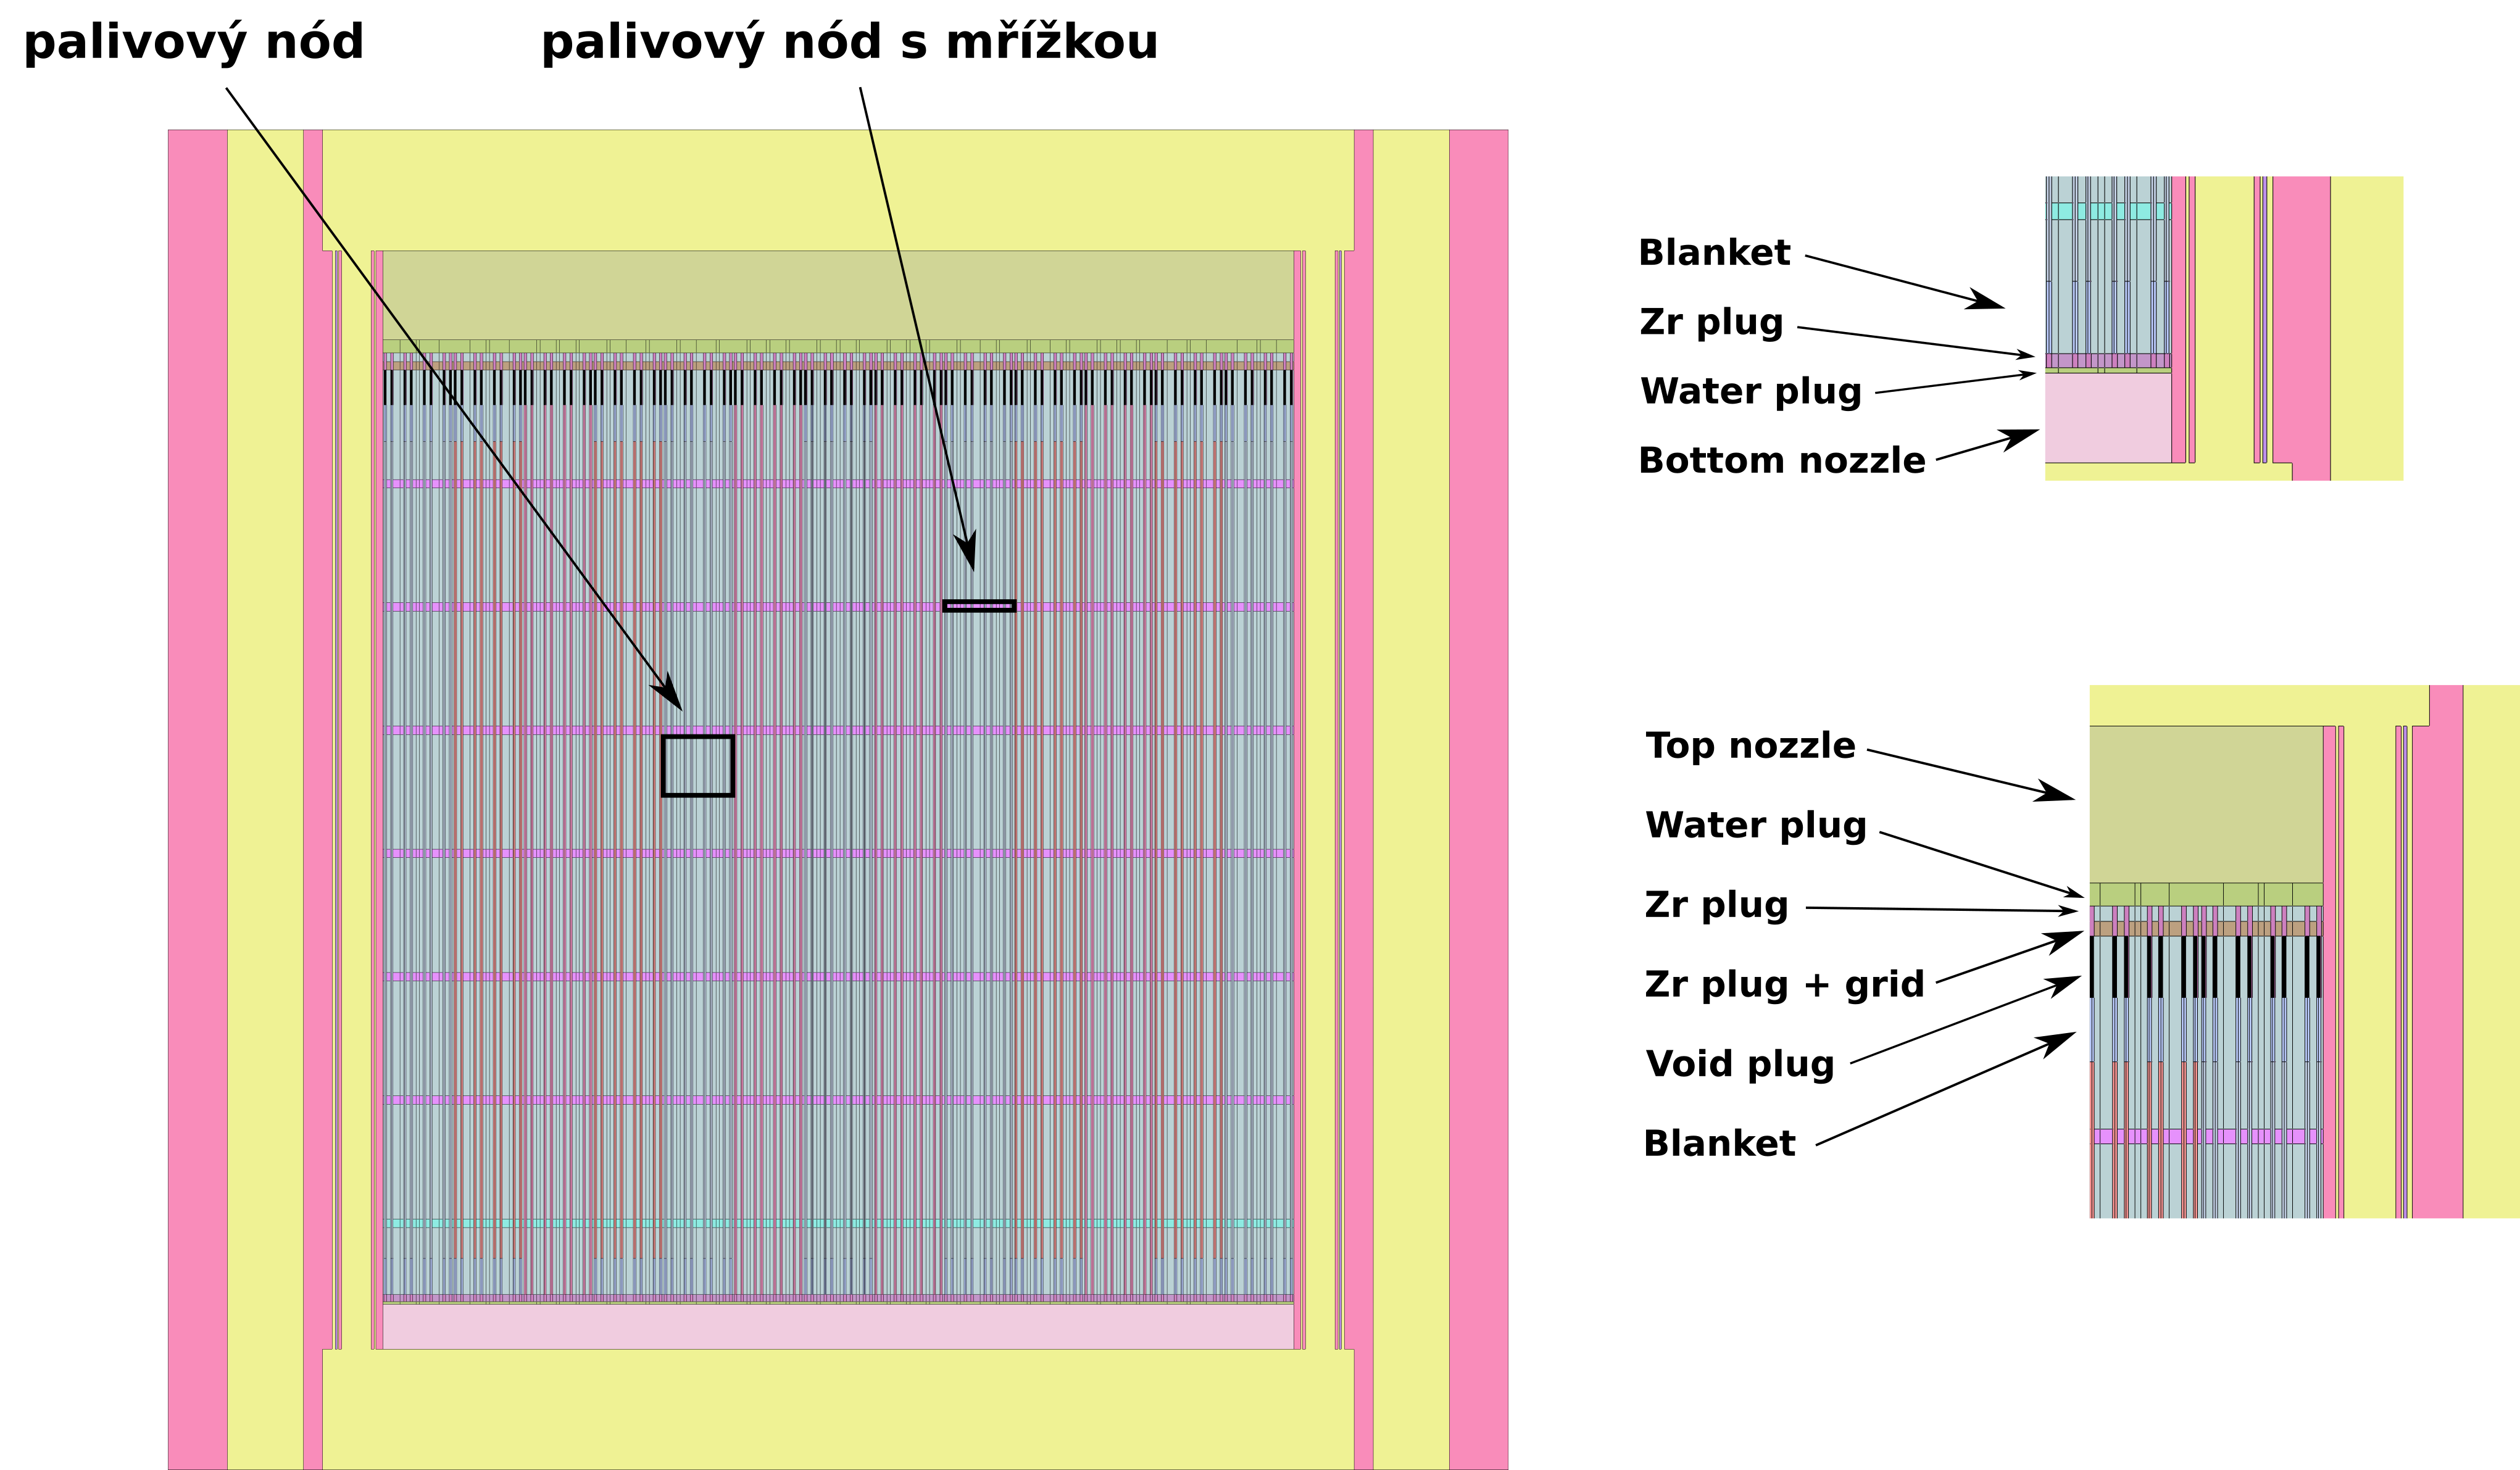
\includegraphics[scale=0.35]{img/reactor_axial_schema.png}
\end{figure}
\end{frame}

\begin{frame}{Výpočet rozložení výkonů na HFP}
\begin{block}{}
\begin{itemize}\scriptsize
	\item rychlost výpočtu rozložení výkonu na HFP je závislá na počtu iterací rozložení výkonu/teplot 
    \item je vhodné mít co nejlepší odhad rozložení teplot v nódech před výpočtem
\end{itemize}

\end{block}

\begin{figure}
	\centering
	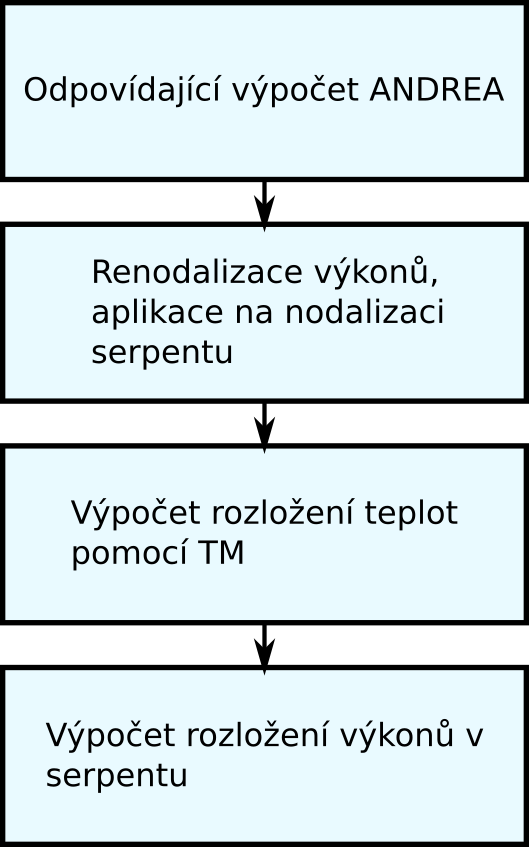
\includegraphics[scale=0.4]{img/vypocet_teploty.png}
\end{figure}
\end{frame}

\begin{frame}{Modelování vyhoření}
	
\begin{block}{}
\begin{itemize}\footnotesize
	\item generický model sestavený na základě vybraných typů kazet 
	\item pouze pro výpočty 'dostatečně' dlouho po odstavení
	\item nelze reprezentovat gradient vyhoření
\end{itemize}
\end{block}
\begin{figure}
	\centering
	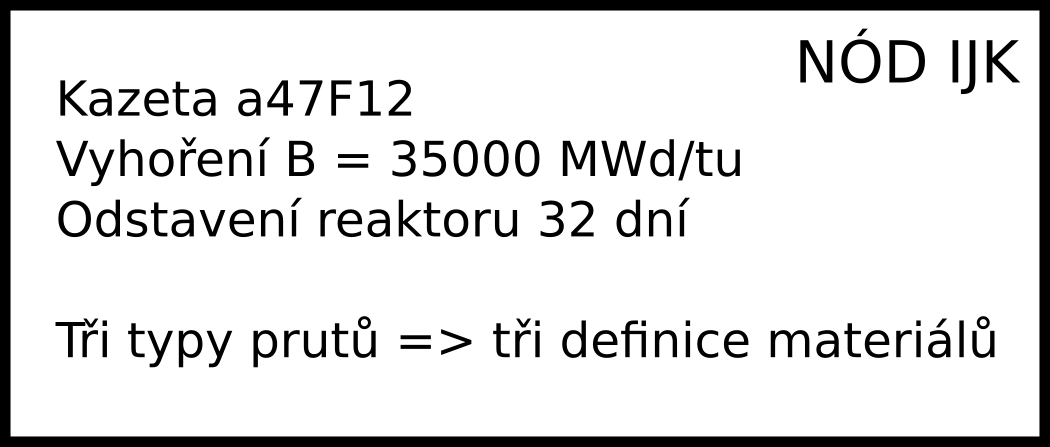
\includegraphics[scale=0.6]{img/nod.png}
\end{figure}
Schéma modelu:\\
    \begin{enumerate}\footnotesize
    	\item na středním výkonu (39 MW/tU) pro několik typů kazet spočteno vyhoření do 75000 MWd/tu a následující odstavení - např. 35 dní
    	\item je vytvořena interpolační tabulka pro koncentrace isotopů v závislosti na vyhoření a počátečním obohacení prutu
    \end{enumerate}
  


	
\end{frame}

\begin{frame}{Vstupní soubor programu SFullcore (1)}
\begin{figure}
	\centering
	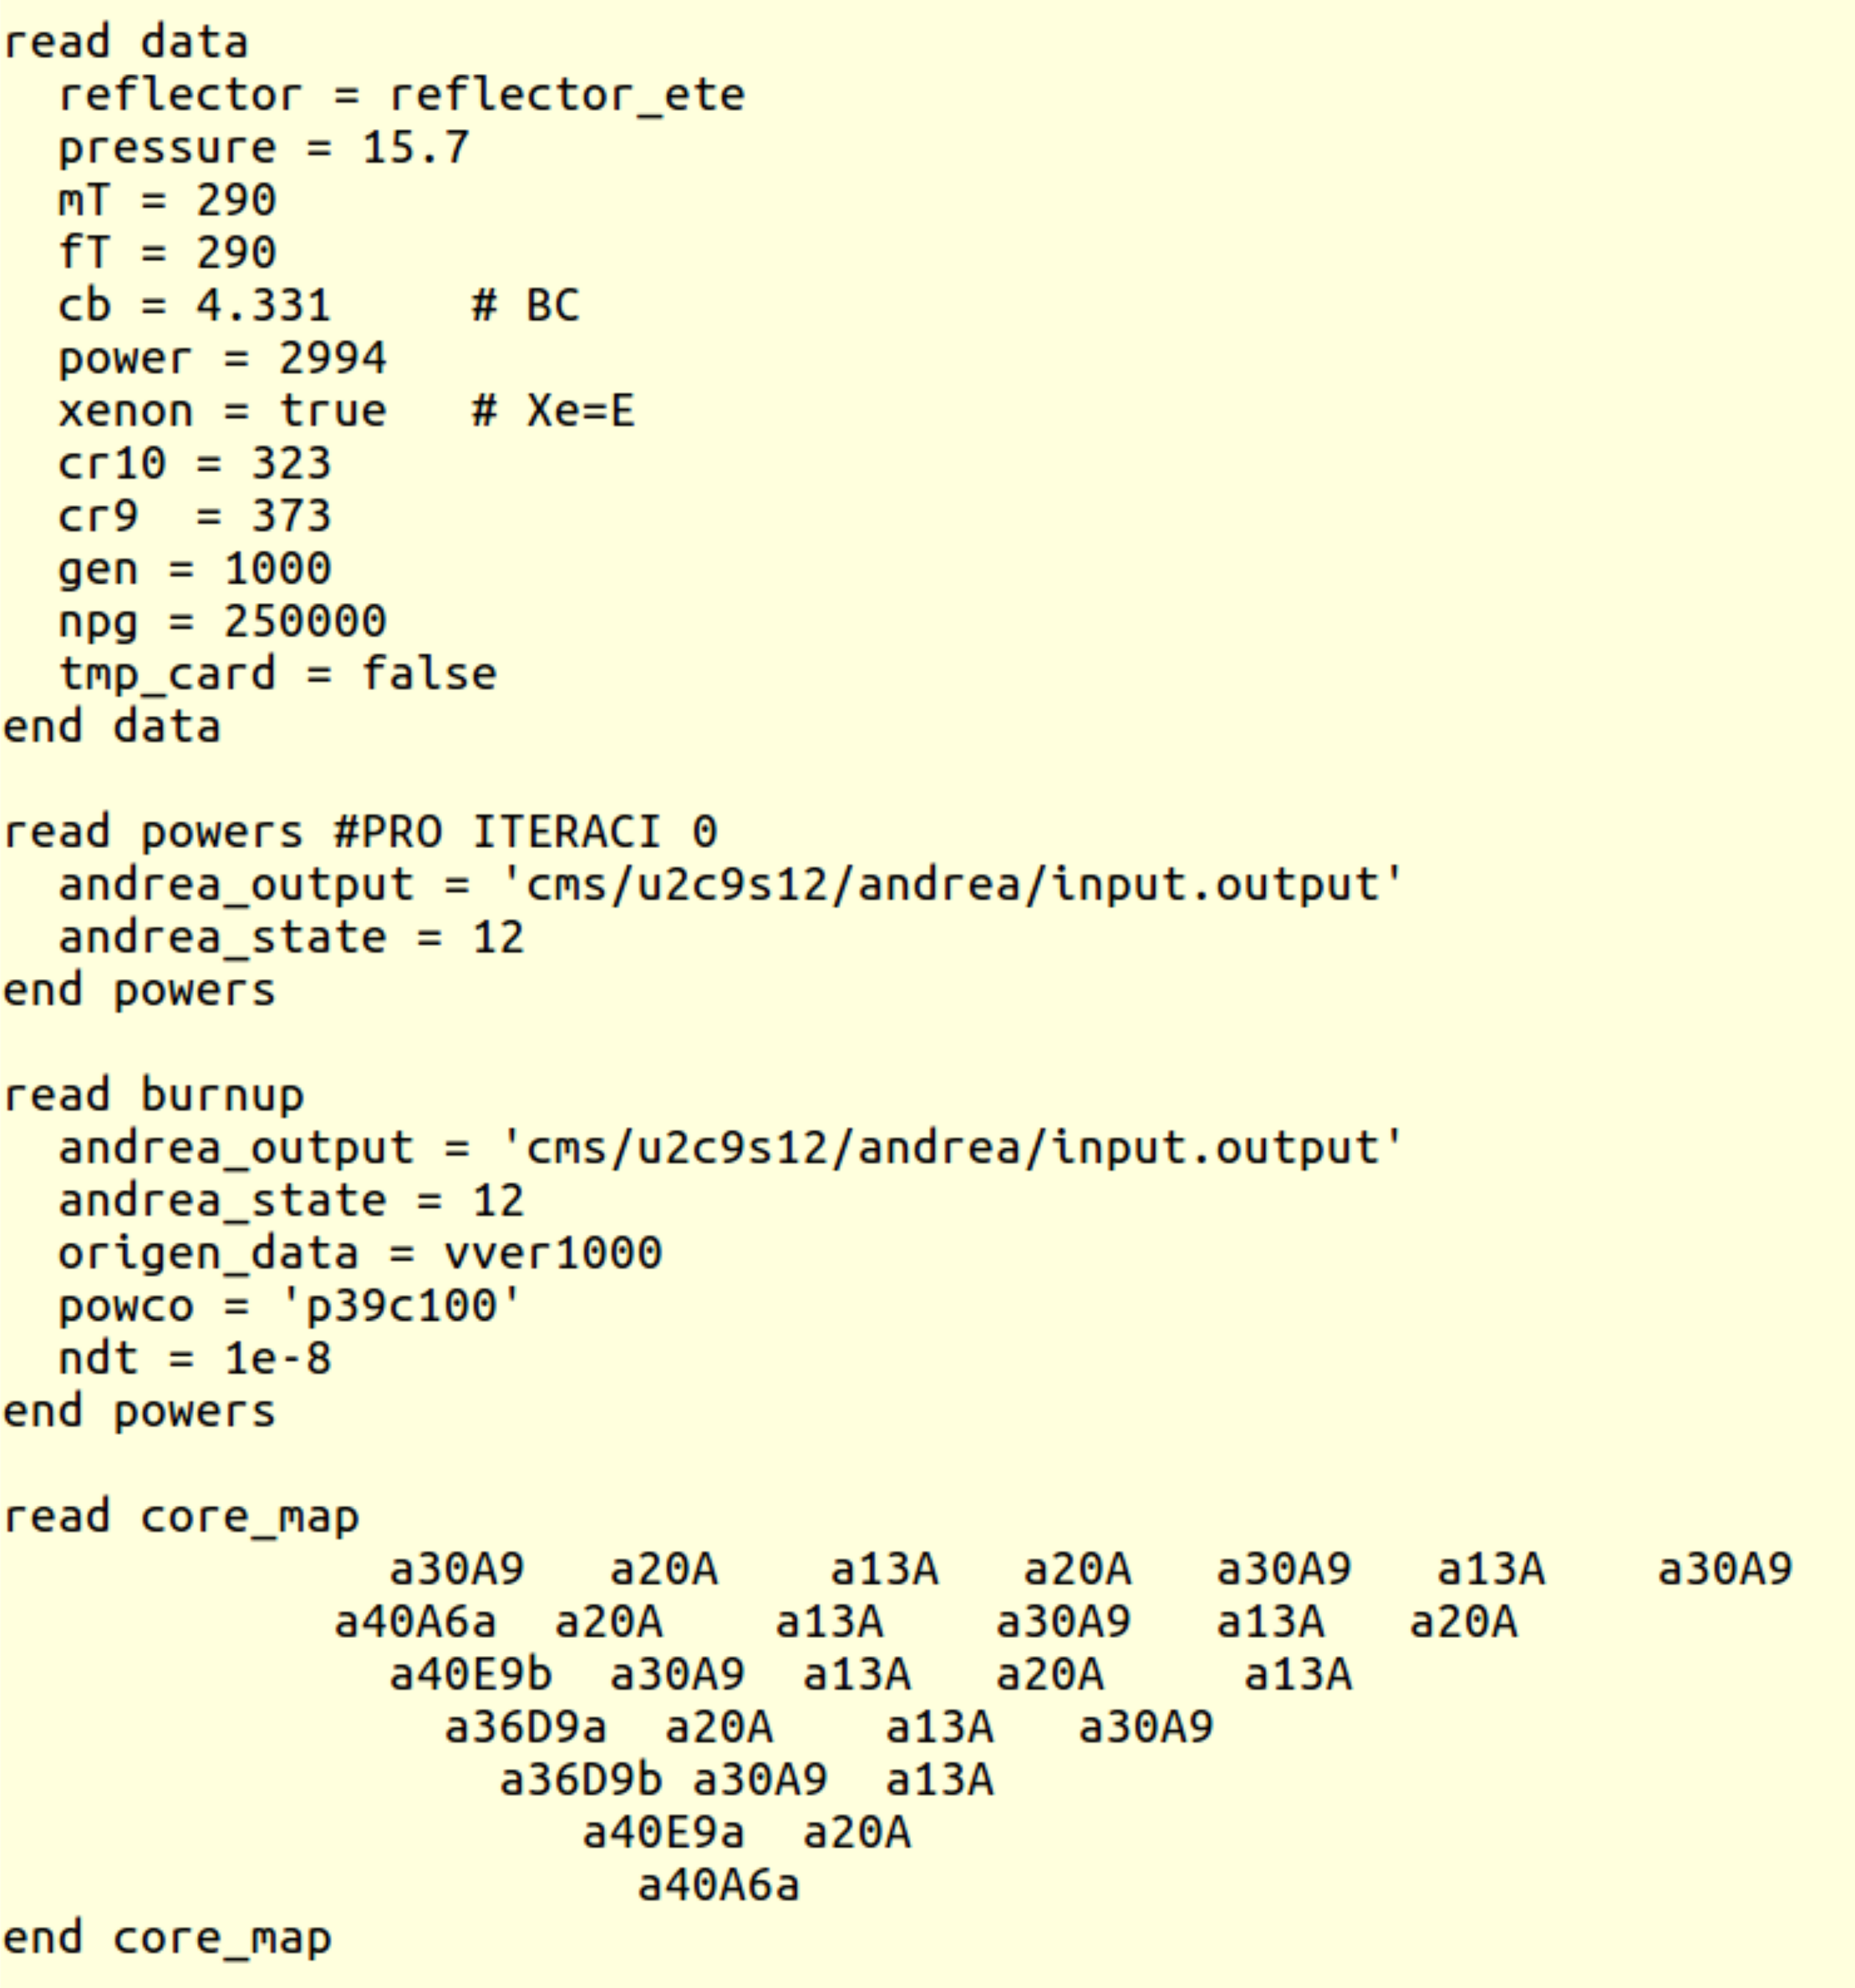
\includegraphics[scale=0.3]{img/input-example1.png}
\end{figure}
\end{frame}

\begin{frame}{Vstupní soubor programu SFullcore (2)}
	\centering
	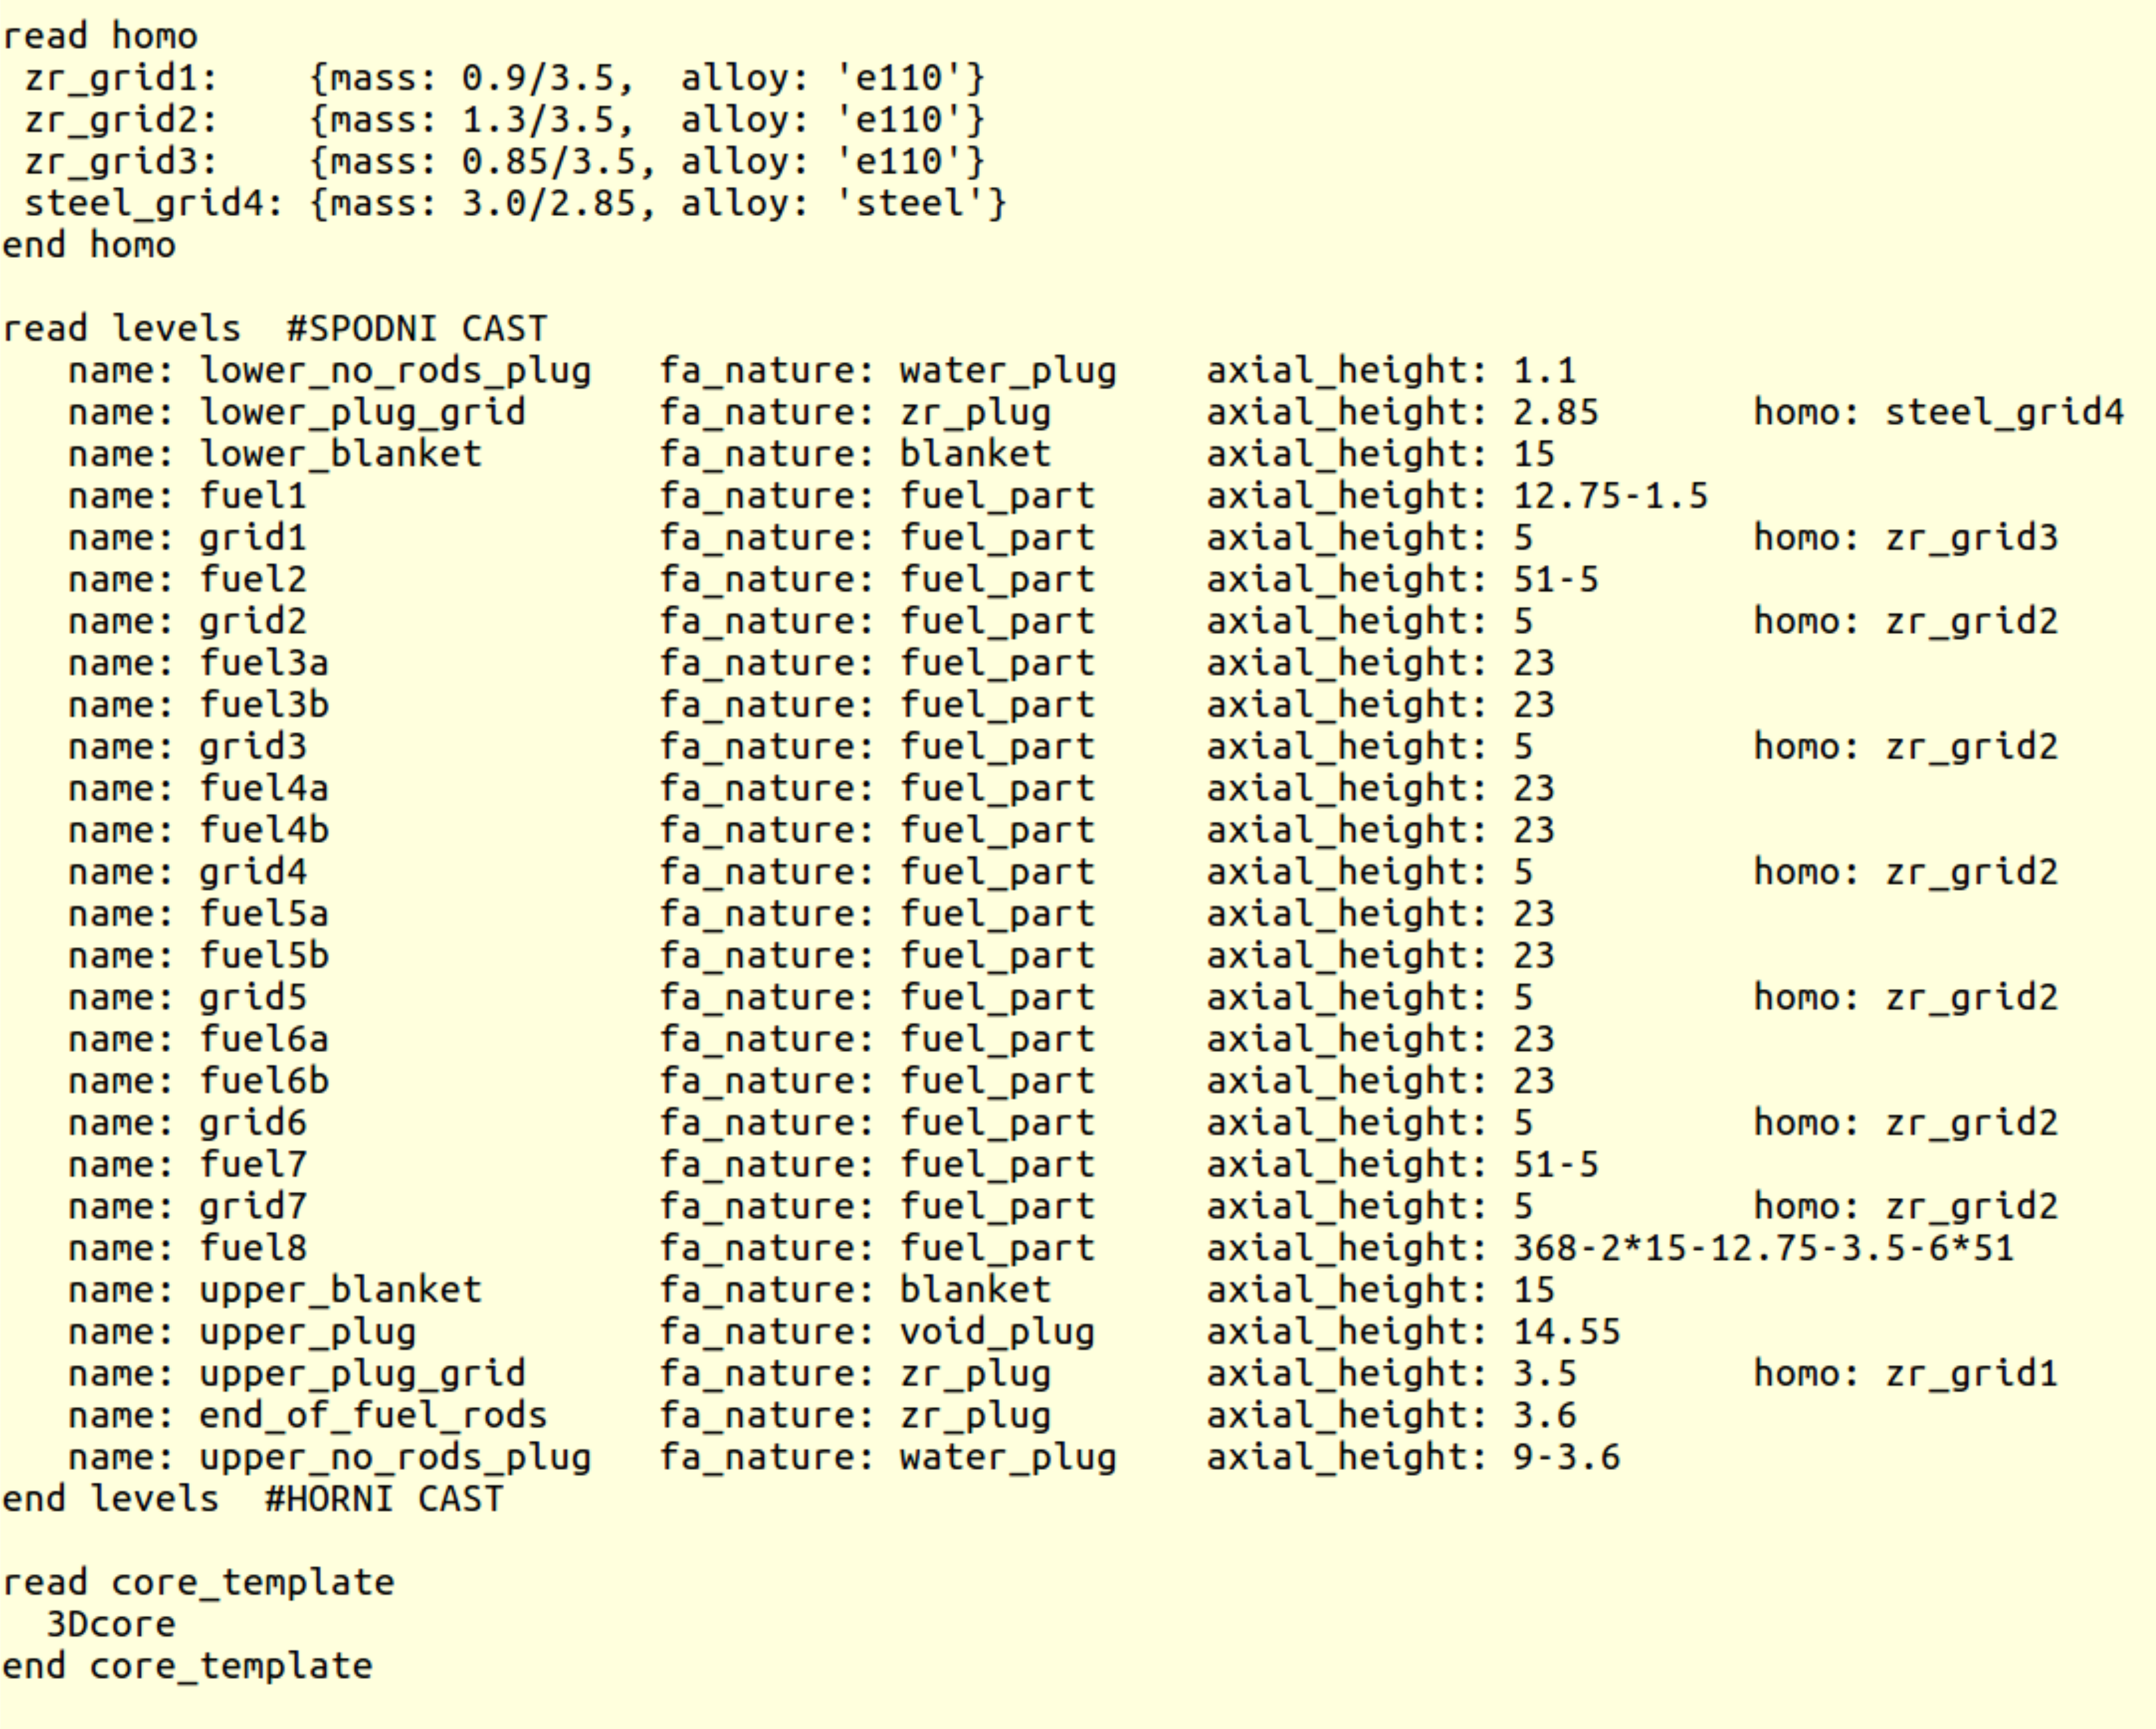
\includegraphics[scale=0.25]{img/input-example2.png}
\end{frame}

%\begin{frame}{Výstupy programu}
%\begin{itemize}\footnotesize
%	\item koeficient násobení
%	\item nodální rozložení neutronových toků (v definové grupové struktuře)
%	\item nodální rozložení definovaných reakčních rychlostí
%\end{itemize}	
%\end{frame}

\section{Porovnaní výpočtů s měřením}


\begin{frame}{Testy spouštění -- F5 ARO}
	
\begin{block}{}\small
	Měření kritické koncentrace kyseliny borité na začátku kampaně
\end{block}

\begin{itemize}\footnotesize
	\item vyhoření predikované programem ANDREA
	\item složení paliva v závislosti na vyhoření předpočteno programem SCALE 
\end{itemize}

\begin{table}[h]\scriptsize
	\begin{center}
		\begin{tabular}{cccc|cccc}
			\toprule
			& CMS     & SERPENT & Rozdíl & & CMS & SERPENT & Rozdíl \\
			\midrule
			\textbf{u1c9      } & 6.59     & 6.58     & -0.02     & \textbf{u2c9      } & 6.69     & 6.59     & -0.10    \\ 
\textbf{u1c10     } & 8.94     & 9.00     & 0.06      & \textbf{u2c10     } & 9.12     & 9.19     & 0.07     \\ 
\textbf{u1c11     } & 10.09    & 10.03    & -0.06     & \textbf{u2c11     } & 8.80     & 8.71     & -0.09    \\ 
\textbf{u1c12     } & 10.02    & 9.93     & -0.09     & \textbf{u2c12     } & 10.54    & 10.48    & -0.06    \\ 
\textbf{u1c13     } & 10.22    & 10.07    & -0.15     & \textbf{u2c13     } & 10.65    & 10.51    & -0.14    \\ 
\textbf{u1c14     } & 0.00     & 0.00     & 0.00      & \textbf{u2c14     } & 9.12     & 9.02     & -0.09    \\ 

			\bottomrule
		\end{tabular}
		\caption{\footnotesize F5 ARO -- kritická kocentrace kys. borité}
	\end{center}
\end{table}
\end{frame}

\begin{frame}{Testy spouštění -- F4 ITC}

\begin{block}{}\small
	Měření izotermického koeficientu reaktivity 
\end{block}

\begin{itemize}\footnotesize
	\item snížení a zvýšení teploty systému o 1.5 $^\circ$C
\large	\item ITC =  $\frac{\textrm{k}_{\textrm{zvýšení}}-\textrm{k}_{\textrm{snížení}}}{
\textrm{3}}$

\footnotesize	\item náročný výpočet z hlediska jeho neurčitosti
\item výsledek negativně ovlivněn velkým rozdílem teplot (3 $^\circ$C)
\end{itemize}

\begin{table}[h]\scriptsize
	\begin{center}
		\begin{tabular}{ccccc}
			\toprule
			& CMS     & SERPENT \tiny min & SERPENT \tiny mean & SERPENT \tiny max\\
			\midrule
			\textbf{u1c9      } & -3.53    & -1.33    & \textbf{-2.67   } & -4.00    \\
\textbf{u2c9      } & -4.50    & -3.33    & \textbf{-4.67   } & -6.00    \\

			\bottomrule
		\end{tabular}
		\caption{\footnotesize F4 ITC}
	\end{center}
\end{table}

\end{frame}

\begin{frame}{Výkonový stav -- E2 (U2C9)}

\begin{block}{}\small
	Test rozložení výkonu kazet (na 100 \% výkonu rektoru)
\end{block}

\begin{table}[h]\scriptsize
	\begin{center}
		\begin{tabular}{ll}
Výpočet & Reálný stav \\			
			\toprule
bez vyhoření & vyhoření cca 3.5 Teff \\
proveden s Xe=E & xenon 'dojíždí' z testu na 80 \% výkonu \\
			\bottomrule
		\end{tabular}
	\end{center}
\end{table}

\begin{itemize}\footnotesize
	\item 'lze' provést korekce na vyhoření a chování xenonu
	\item korekce na BC: cca 0.2 g/kg BC

\end{itemize}
	
\begin{table}[h]\scriptsize
	\begin{center}
		\begin{tabular}{cccc}
			\toprule
			& CMS    & SERPENT (\tiny Teff = 0) & SERPENT (\tiny Teff = 3.5) \\
			\midrule
			\textbf{u2c9/e2   } & 4.331    & 4.524    & 4.315   \\

			\bottomrule
		\end{tabular}
		\caption{\footnotesize Kritcká BC měření E2}
	\end{center}
\end{table}
\end{frame}




\begin{frame}{Výkonový stav -- U2C9/S12 (mapa)}
	\begin{figure}[!h]
		\centering
		%       \includegraphics[scale=0.15]{../img/fha__4_full_S4.pdf}
		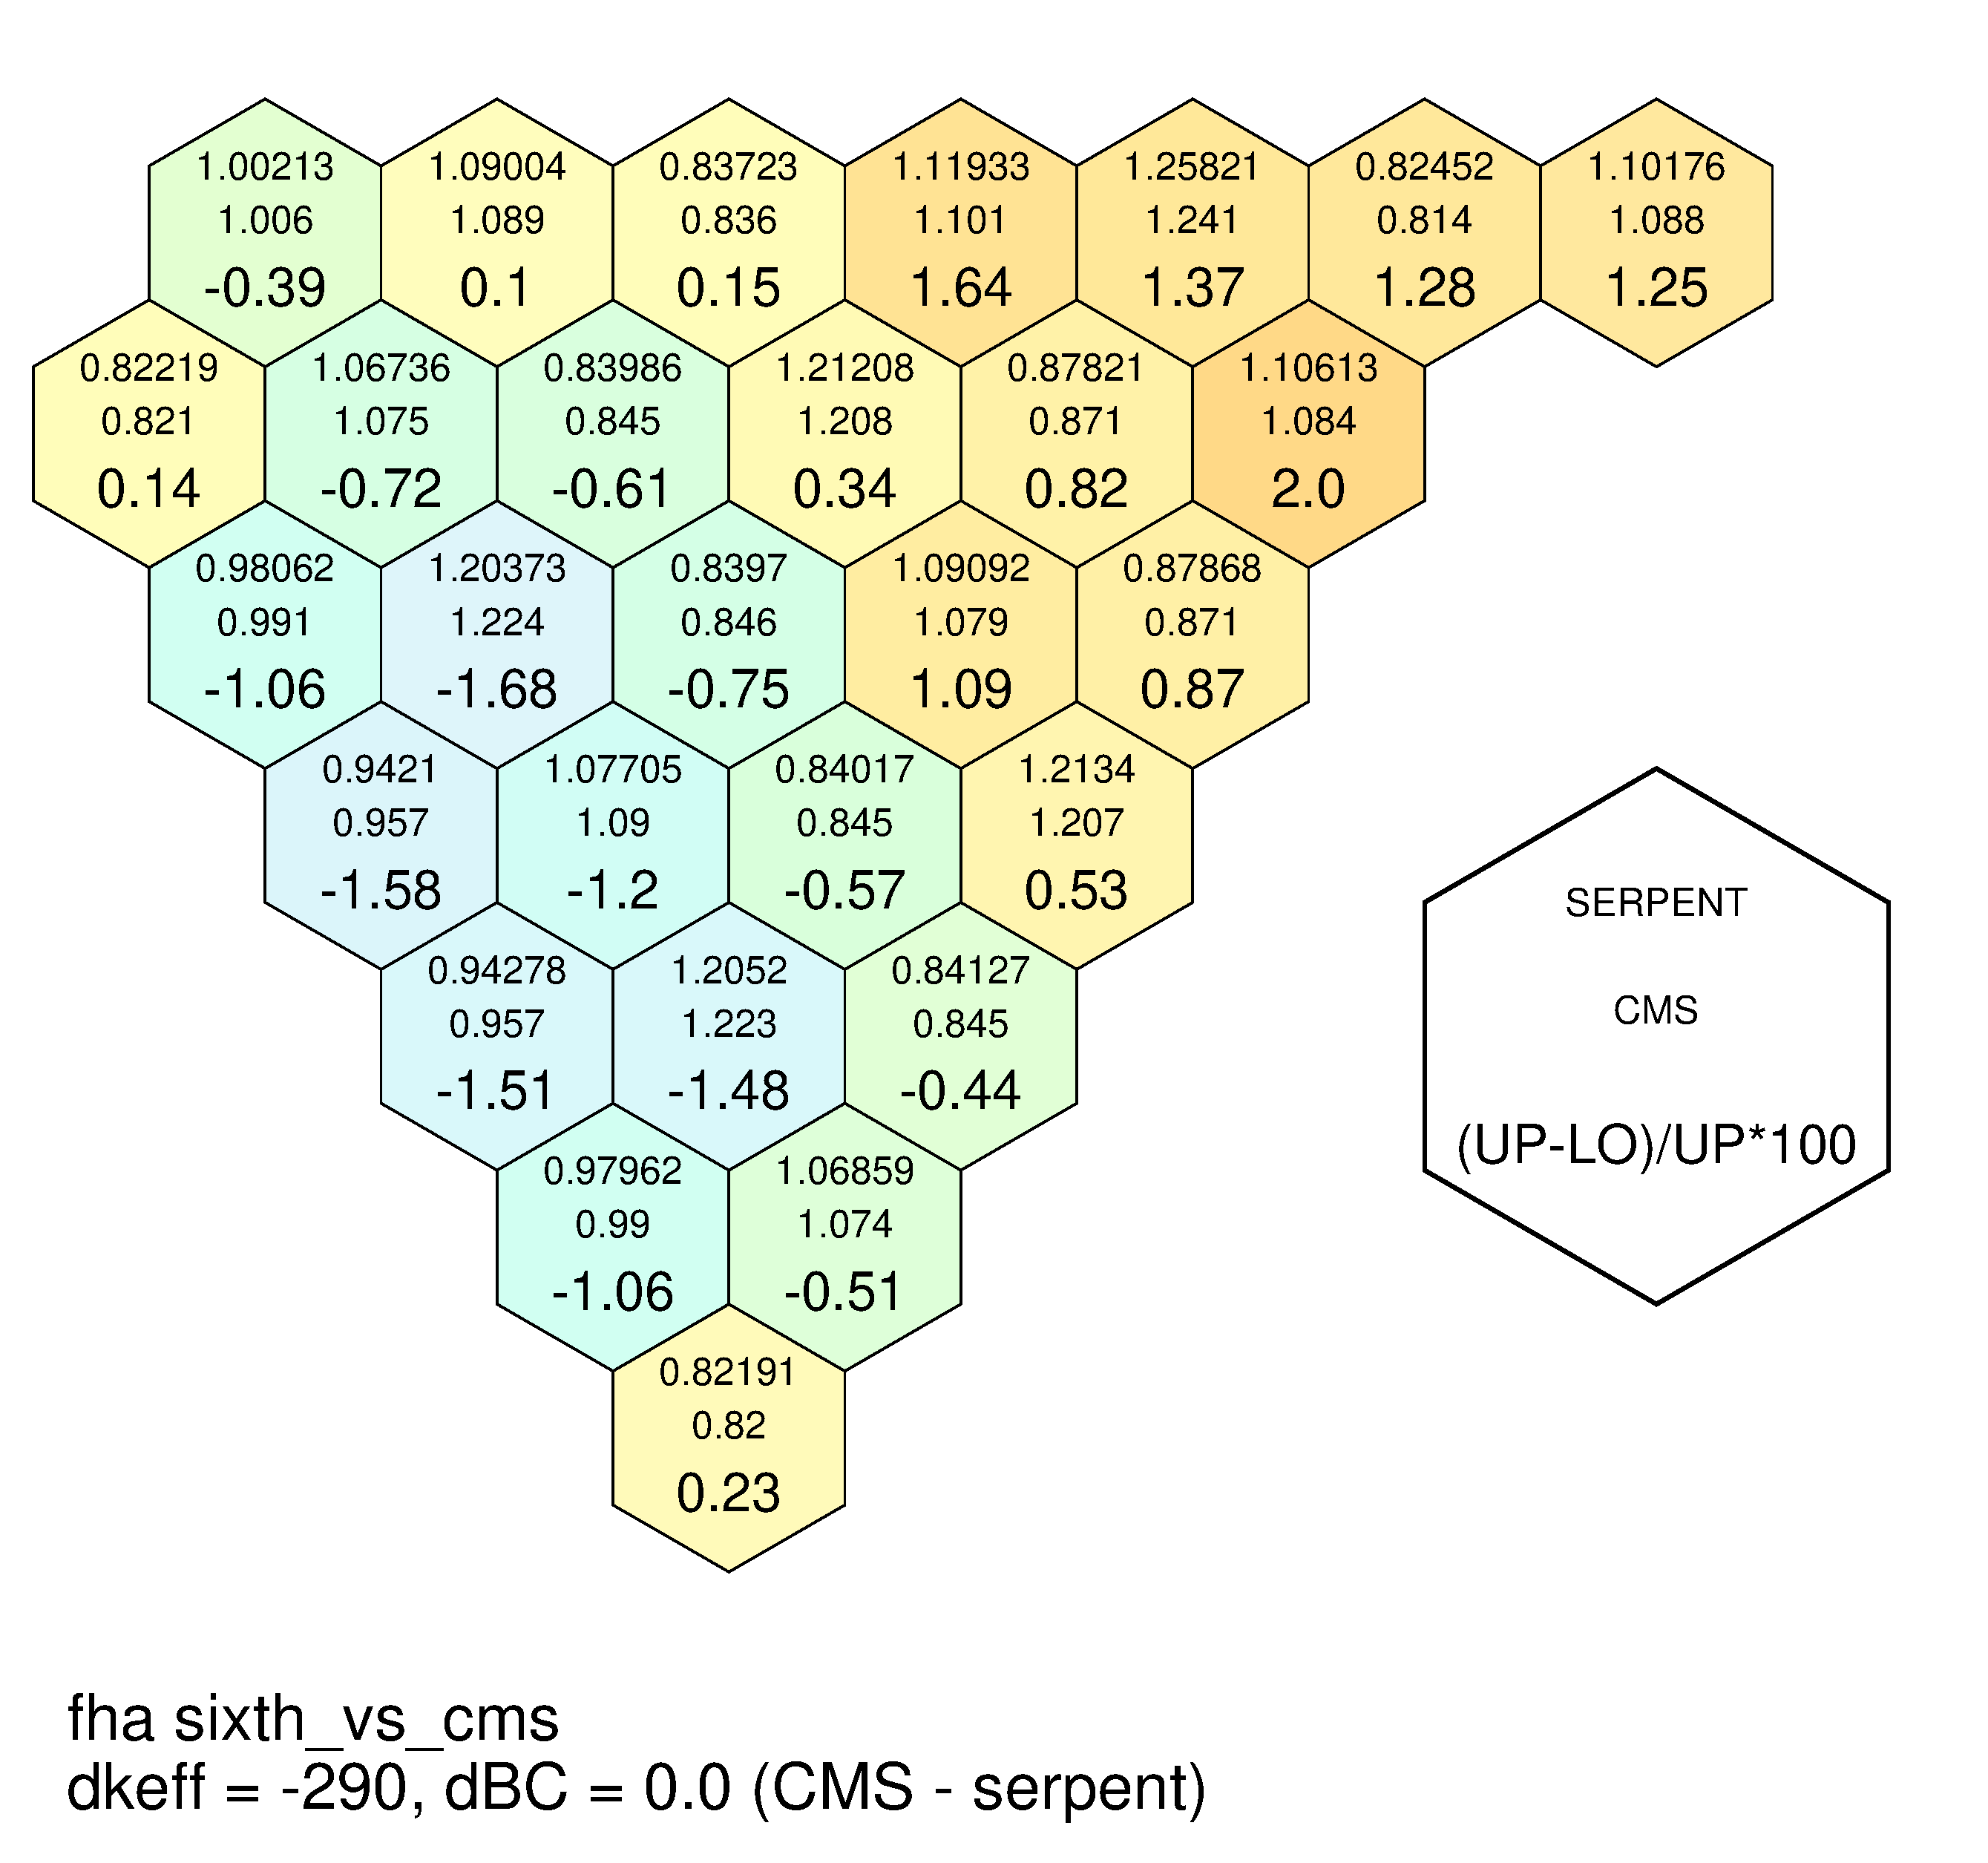
\includegraphics[scale=0.13]{img/fha_sixth_vs_cms.pdf}
		\caption{\footnotesize Srovnání SERPENT - CMS}
		%       \caption{Srovnání SERPENT - CMS (nahoře), srovnání ANDREA - CMS (dole)}
	\end{figure}
\end{frame}

\begin{frame}{Výkonový stav -- U2C9/S12 (mapa)}
	\begin{figure}[!h]
		\centering
		%       \includegraphics[scale=0.15]{../img/fha__4_full_S4.pdf}
		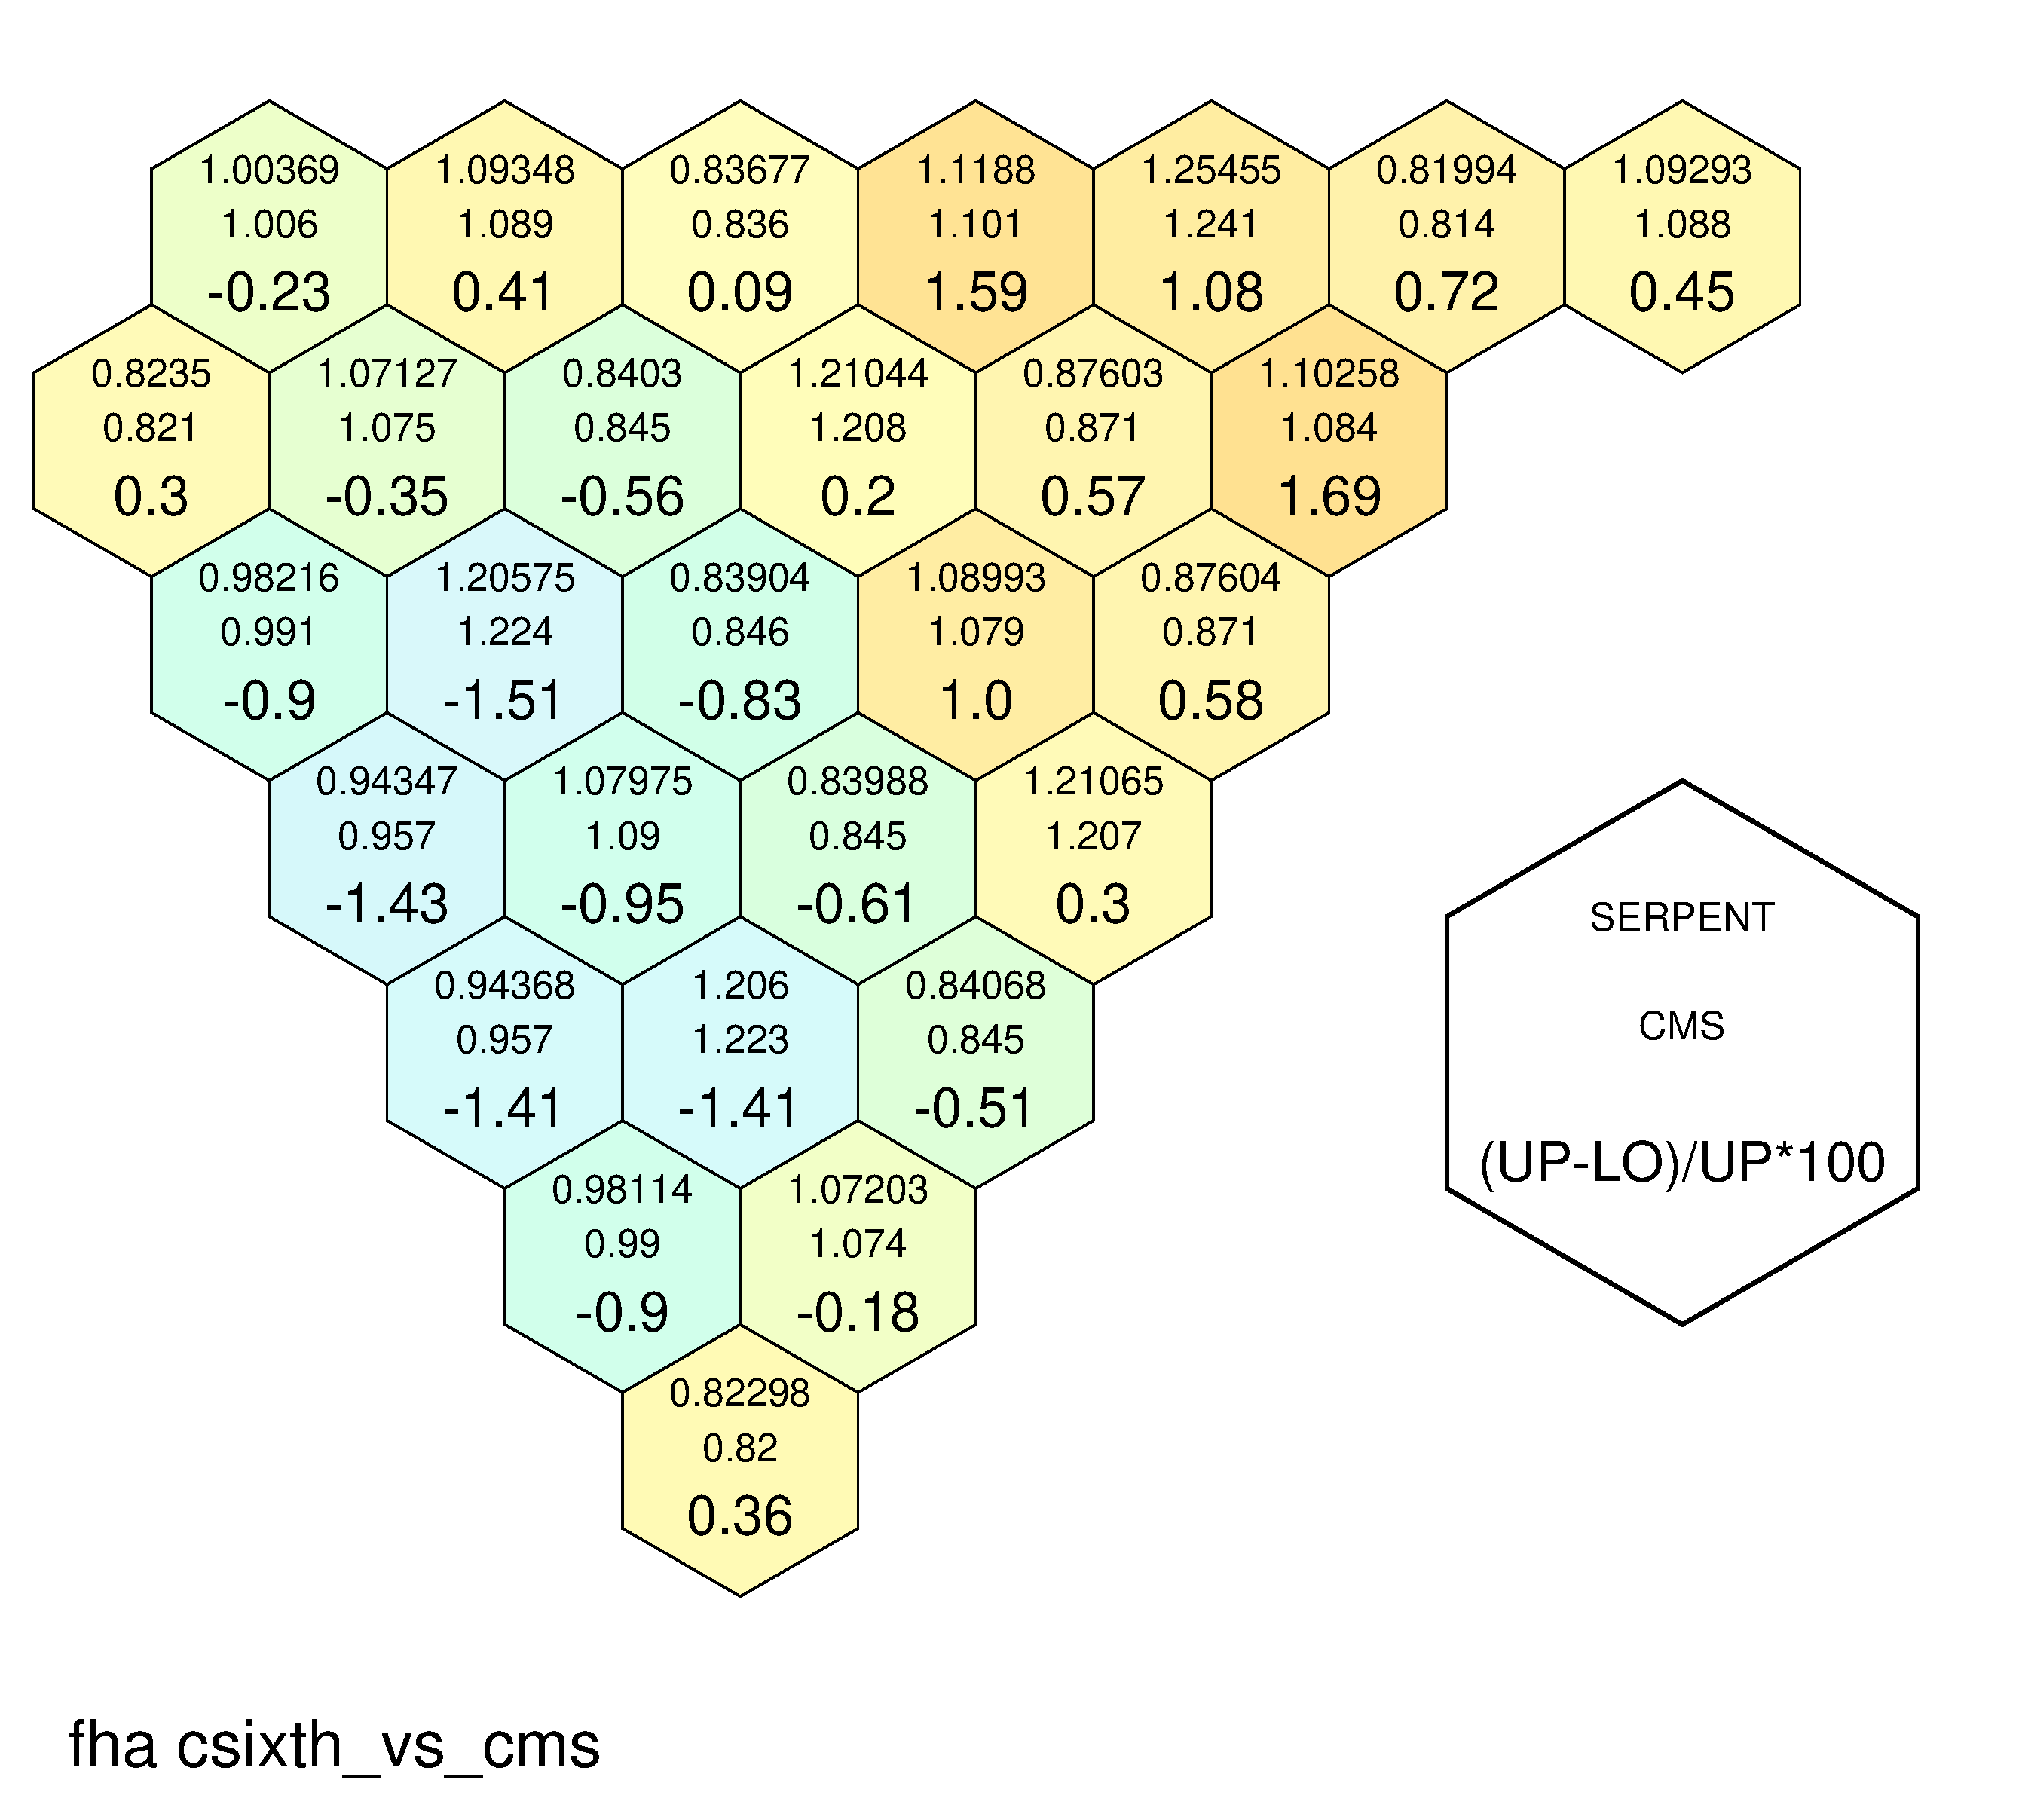
\includegraphics[scale=0.13]{img/fha_csixth_vs_cms.pdf}
		\caption{\footnotesize Srovnání SERPENT - CMS (korekce na vyhoření)}
		%       \caption{Srovnání SERPENT - CMS (nahoře), srovnání ANDREA - CMS (dole)}
	\end{figure}
\end{frame}


\section{Závěrem}

\begin{frame}{Závěrem}
	\begin{itemize}
		\item Zlepšení modelu vyhoření kazet 
		\item Pokus o výpočet na HFP s vyhořením reaktoru
	\end{itemize}
\end{frame}


\end{document}
